\documentclass{article}
\usepackage[utf8]{inputenc}

\title{ERSS HWK4 Scalability}
\author{Chenfan Li(cl414) You Lyu (yl489)}
\date{April 2018}

\usepackage{natbib}
\usepackage{graphicx}
\usepackage{indentfirst}

\begin{document}

\maketitle

\section{Methodology}
This matching server is implemented in C++ language. To improve the system scalability, thread pool from boost library is used.\vspace{\baselineskip}

The basic idea is to break up multiple “tasks”, which in this case is the order operation indicated by each child of <transaction> root node in transaction XML. For example, if a transaction XML request has two <order> tags and a <query> tag, then each of them will be a separate task (as the requirement indicates, children nodes of a transaction root node can be handled in any order). To be specific, each child node operation, like <query> and <cancel> will be considered as a task, and the task will be assigned to a particular thread which is previously created and managed in a thread pool class. After a thread finishes its work, it will return to idle state and waiting for another task to be assigned. In other word, this matching server is implemented using a “task parallel” philosophy.\vspace{\baselineskip}

As all accounts, unfinished order and order records are stored in the database, the purpose of this design methodology is to reduce the potential IO latency occurred during the query and update of database. As most operations related to databases will be in each child node operation of <transaction> root node, many of them will be paralleled as they are executed in different threads and possibly in different cores.
Note that if a request has a <create> root node, the child nodes will be handled in the order they came in, so no other thread will be assigned to a child node of <create>.

\section{Testing and Results}
The server system is tested in a machine with four two-core processors. To analyze the scalability of this server, special test suites have been developed. The detailed testing methodology can be found in the README document in ./testing sub directory.
\subsection{Fixed Competing Requests with Different Computing Resources}
Concisely speaking, in the first set of tests, the varying factor “competing request” is fixed. In this case, the peek number of competing requests will be in 1000 level. To test the scalability of this system, the number of computing resources will be a variable.\vspace{\baselineskip}

The tests used 1, 2, 4, 8 and 16 threads (number of threads in the thread pool) to represent the increased computing resources (will be demonstrated as X axis in the graph) as the machine which used to conduct the testing has multiple cores.\vspace{\baselineskip}

The results in Y axis represents the time spent to finish handling one request (from receiving the request to finishing sending response). Note that the contents of requests sent concurrently for testing are from two different .xml input files, each of them contains operations including <order> (both sell and buy), <query> and <cancel> to simulate multiple transaction operations.\vspace{\baselineskip}

This testing is basically to send more than a thousand requests at a time and the server will count the time interval (in micro seconds) used for each completed request handling.\vspace{\baselineskip}

The tests are conducted for more than 20 times and the average values of multiple set of time interval data are used for graphing. The testing results are shown as Figure 1 with error bars.


\begin{figure}[h!]
\centering
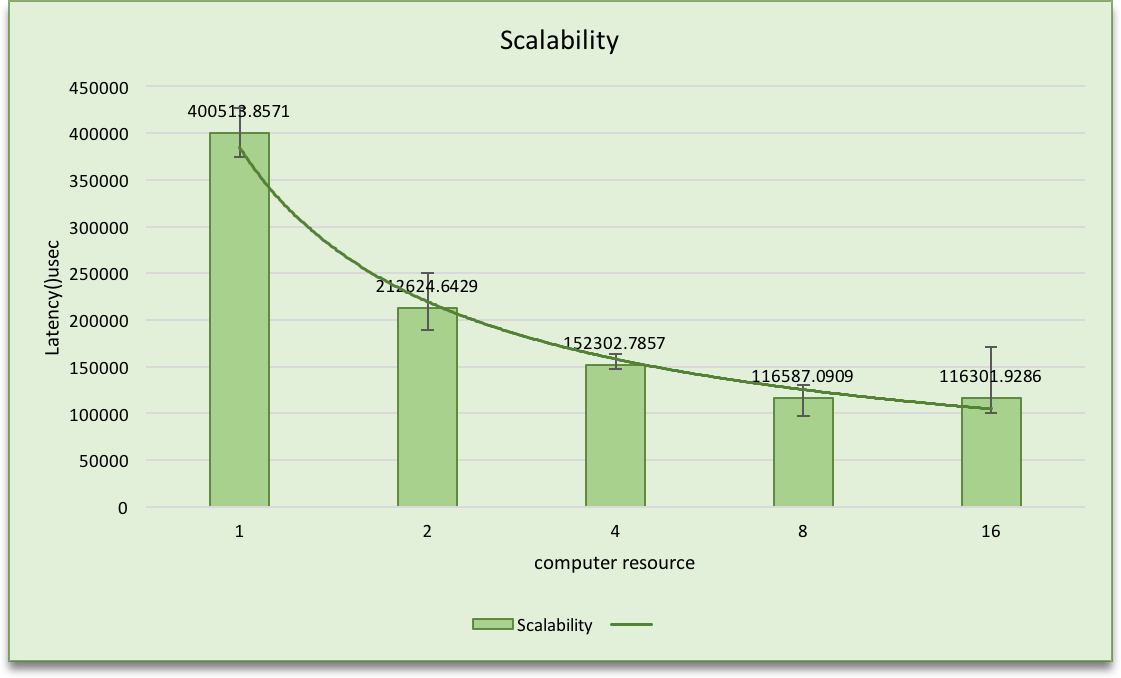
\includegraphics[scale=0.5]{ece5902.png}
\caption{Task Latency for Fixed Competing Requests with Different Computing Resources of Matching Server}
\label{fig:universe}
\end{figure}

\subsection{Fixed Computing Resources with Different Competing Requests}
In the second set of tests, computing resources (in this case the number of threads in the thread pool) will be fixed, in this case 8 threads, and the variable will be competing requests.\vspace{\baselineskip}

For testing purpose, the number of requests sent at a time (demonstrated as X axis values for graphing) will be changed from 2 to 10 to 100 and to more than 1000 (with different suites). The Y axis will be the longest time or latency for the “client” who sent the requests to receive a response. Note that during the testing, the time used to represent “latency” is counted on the client side. The latency value will be the time interval (in micro seconds) for a certain request to get its response.\vspace{\baselineskip}

The testing is basically to send different number of requests (containing multiple operations) at a time and calculate the longest latency on the client side. The tests are conducted for more than 20 times and the average values of multiple set of time interval data are used for graphing. The testing results are shown as Figure 2 with error bars.

\begin{figure}[h!]
\centering
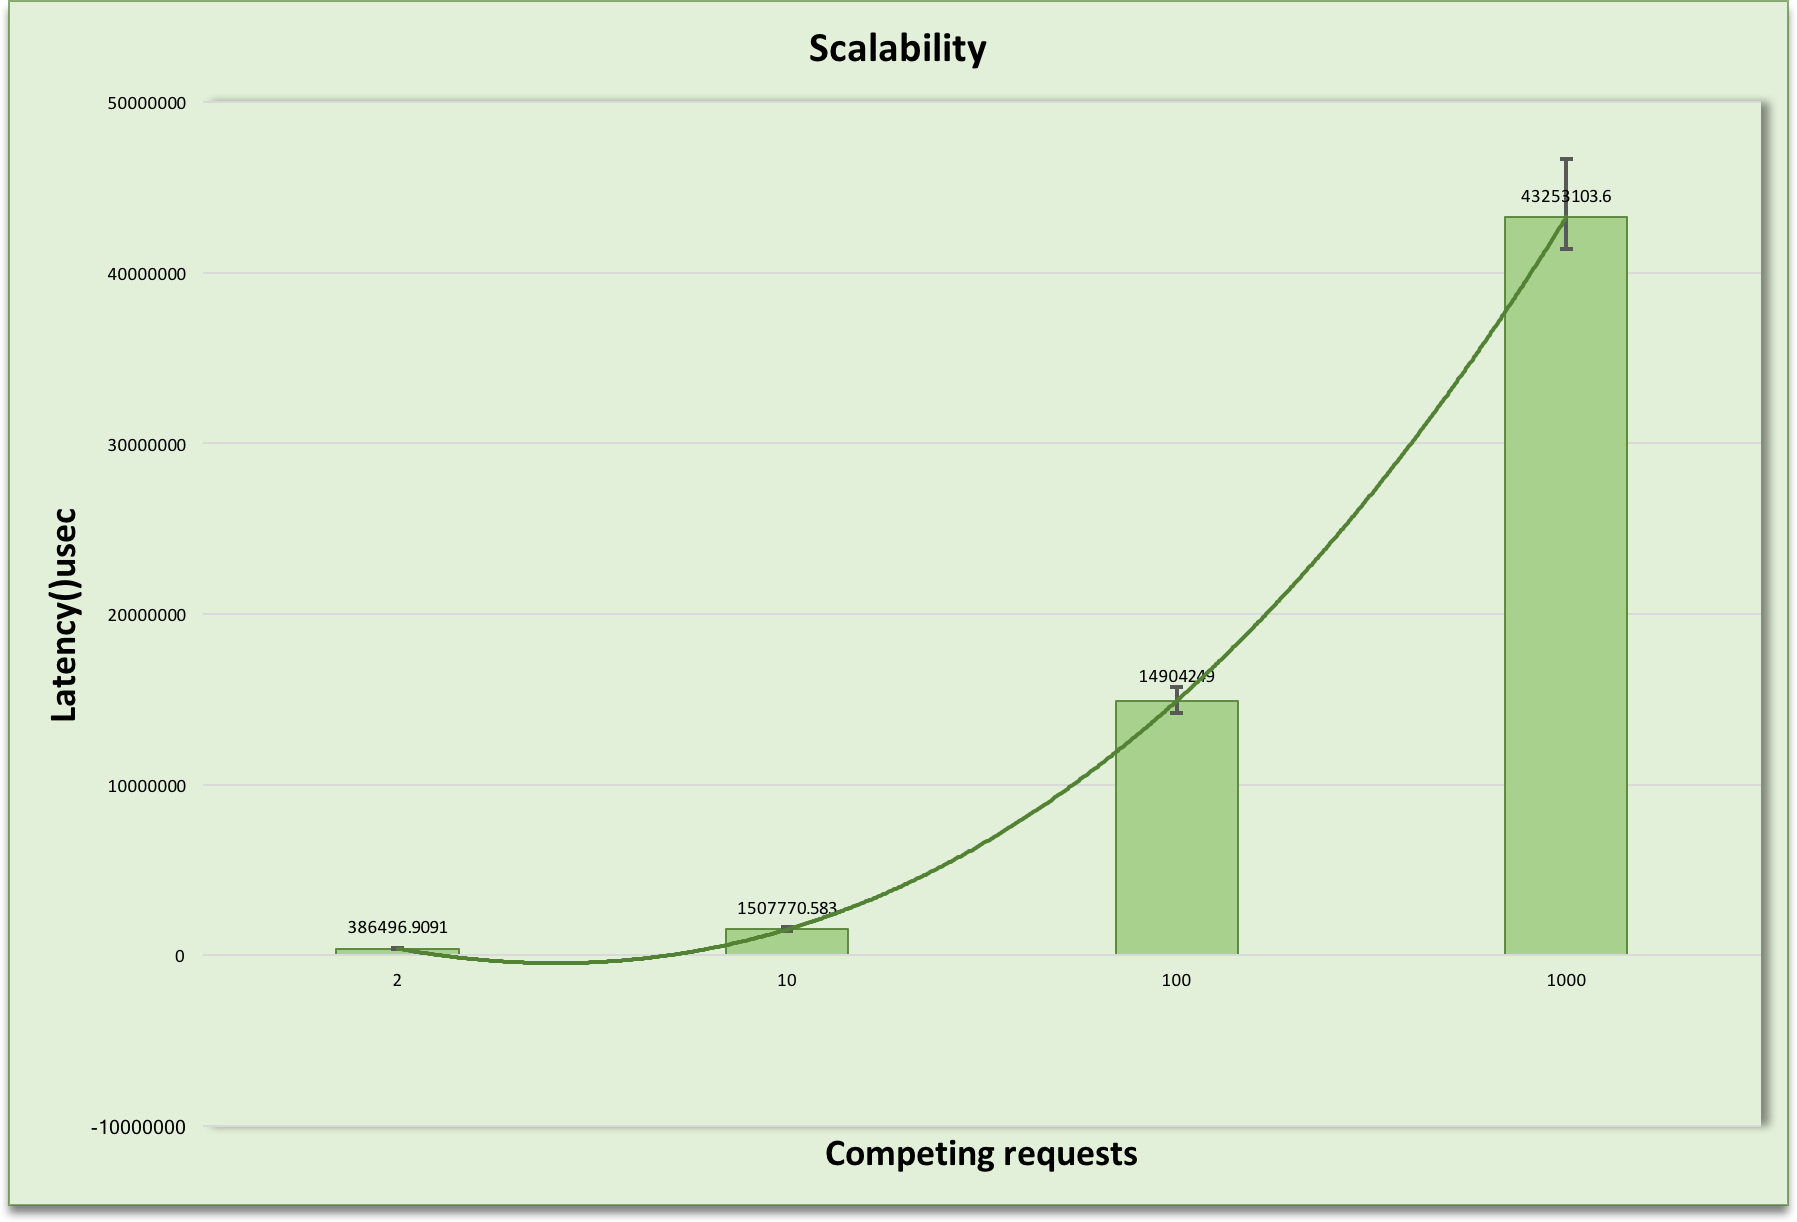
\includegraphics[scale=0.3]{ece5901.png}
\caption{Request Latency for Fixed Competing Requests with Different Computing Resources of Matching Server}
\label{fig:}
\end{figure}

\section{Scalability Analysis}
From Figure 1, it can be seen that with the amount of computing resources increasing, the time required to finish each task (latency) will decrease. Specifically, when the number of thread increase from one thread to two threads, the average time required to handle each task will be nearly halved. This means that the task has been well paralleled in two units of computing resources. When the computing resource is doubled from 2 to 4, the amount of latency will decrease about 28.4\%. When the computing resource is doubled from 4 to 8, the amount of latency will decrease about 23.5\%.\vspace{\baselineskip}

Generally, it can be observed that the server has a certain level of scalability which is indicated by the improvement of performance with the increase of computing resources. However, while the ideal model is when the computing resource doubled, the latency to perform each task will be halved, the server’s actual performance will be limited by its serialized part.\vspace{\baselineskip}

In this design, all the unfinished orders, executed and canceled orders as well as the user account will be stored to the database. PostgreSQL is used as the database of this design and there are many levels of locks in its design to prevent lost of synchronization while more transactions are altering a certain row of data. The multi-level locks and other synchronization implementations in PostgreSQL will be one of the major serialized parts that limit the parallel performance.\vspace{\baselineskip}

Apart from that, in order to response each <transaction> and <create> operation properly, each assigned thread to handle a certain task will be expected to modify a shared data structure called “response”. To prevent loss of synchronization and data race, mutex lock and lock guard in STL are used to protect the writing of “response”. This lock can also place impediment on server’s parallel performance.\vspace{\baselineskip}

Also, as threads are assigned to different tasks, the “parent” thread which spawns new threads will need to wait until all its children have finished handling the tasks. In this implementation, “join” method from thread pool is used. This indicates that the task which take longest time to finish will be the “critical path” of the whole request handling process. This may also be an implication of load balancing where better methodology may assign the task on a more balanced manner. In other words, improve the load balancing may be a good way of improving system’s scalability.\vspace{\baselineskip}

From Figure 2, it can be observed that with the number of competing requests increasing, the latency, which is counted as the longest response time of a certain request, will increase considerably in a nearly quadratic manner. While the increasing of latency’s rate of change seems normal as the scale changes from 2 to more than 1000, that rate of change could be limited in several possible ways.\vspace{\baselineskip}

One important consideration is load balancing, although the system performs well when handling multiple concurrent tasks, the load balancing of the system needs to be improved. If parallel performance of the system is good, then adding computing resources may be a good way of handling increasingly large amounts of requests.\vspace{\baselineskip}

In addition, as there are more requests coming, more data is likely to be stored in the database. As it seems common, SQL queries may take longer to finish as more lookup and matching will be performed. The actual system may set expiration examination to kick out expired order to maintain the total amount of the data or use separate storage tables or databases to classify and store different types of data. These implementations may improve the scalability of the system for handling increasingly large amounts of competing requests (real systems like Taobao double eleven sever could be a good study material for that).

\end{document}
